\documentclass[12pt]{article}
\usepackage[utf8]{inputenc}
\usepackage{geometry}
\geometry{letterpaper, margin=0.25in}
\usepackage{graphicx} 
\usepackage{parskip}
\usepackage{booktabs}
\usepackage{array} 
\usepackage{paralist} 
\usepackage{verbatim}
\usepackage{subfig}
\usepackage{fancyhdr}
\usepackage{sectsty}
\usepackage[shortlabels]{enumitem}

\pagestyle{fancy}
\renewcommand{\headrulewidth}{0pt} 
\lhead{}\chead{}\rhead{}
\lfoot{}\cfoot{\thepage}\rfoot{}

%%% ToC (table of contents) APPEARANCE
\usepackage[nottoc,notlof,notlot]{tocbibind} 
\usepackage[titles,subfigure]{tocloft}
\renewcommand{\cftsecfont}{\rmfamily\mdseries\upshape}
\renewcommand{\cftsecpagefont}{\rmfamily\mdseries\upshape} %

\usepackage{amsmath}
\usepackage{amssymb}
\usepackage{mathtools}
\usepackage{empheq}
\usepackage{xcolor}
\usepackage{bbm}
\usepackage{tikz}
\usepackage{pgfplots}
\usepackage{tikz-cd}
\pgfplotsset{compat=1.18}
\usetikzlibrary{intersections, calc, decorations.markings}
\tikzset{
    marking along/.style n args={2}{
        decoration={
                markings, 
                mark=at position #1 with {\arrow{#2}}
        },
        postaction={decorate}
        },
    marking along/.default={0.5}{>}
}

\newcommand{\ans}[1]{\boxed{\text{#1}}}
\newcommand{\vecs}[1]{\langle #1\rangle}
\renewcommand{\hat}[1]{\widehat{#1}}

\renewcommand{\P}{\mathbb{P}}
\newcommand{\R}{\mathbb{R}}
\newcommand{\E}{\mathbb{E}}
\newcommand{\Z}{\mathbb{Z}}
\newcommand{\N}{\mathbb{N}}
\newcommand{\Q}{\mathbb{Q}}
\newcommand{\C}{\mathbb{C}}

\newcommand{\ind}{\mathbbm{1}}
\newcommand{\qed}{\quad \blacksquare}

\newcommand{\brak}[1]{\left\langle #1 \right\rangle}
\newcommand{\bra}[1]{\left\langle #1 \right\vert}
\newcommand{\ket}[1]{\left\vert #1 \right\rangle}

\newcommand{\abs}[1]{\left\vert #1 \right\vert}
\newcommand{\mfX}{\mathfrak{X}}
\newcommand{\ep}{\varepsilon}

\newcommand{\Ec}{\mathcal{E}}
\newcommand{\A}{\mathcal{A}}
\newcommand{\F}{\mathcal{F}}
\newcommand{\Cc}{\mathcal{C}}
\newcommand{\B}{\mathcal{B}}
\newcommand{\M}{\mathcal{M}}
\newcommand{\X}{\chi}
\renewcommand{\L}{\mathcal{L}}

\newcommand{\sub}{\subseteq}
\newcommand{\st}{\text{ s.t. }}
\newcommand{\card}{\text{card }}
\renewcommand{\div}{\vspace*{10pt}\hrule\vspace*{10pt}}
\newcommand{\surj}{\twoheadrightarrow}
\newcommand{\inj}{\hookrightarrow}
\newcommand{\biject}{\hookrightarrow \hspace{-8pt} \rightarrow}
\renewcommand{\bar}[1]{\overline{#1}}
\newcommand{\overcirc}[1]{\overset{\circ}{#1}}
\newcommand{\diam}{\text{diam }}

\renewcommand{\Re}{\text{Re}\,}
\renewcommand{\Im}{\text{Im}\,}
\newcommand{\sign}{\text{sign}\,}

\newcommand*{\tbf}[1]{\ifmmode\mathbf{#1}\else\textbf{#1}\fi}

\usepackage{tcolorbox}
\tcbuselibrary{breakable, skins}
\tcbset{enhanced}
\newenvironment*{tbox}[2][gray]{
    \begin{tcolorbox}[
        parbox=false,
        colback=#1!5!white,
        colframe=#1!75!black,
        breakable,
        title={#2}
    ]}
    {\end{tcolorbox}}

\newenvironment*{exercise}[1][red]{
    \begin{tcolorbox}[
        parbox=false,
        colback=#1!5!white,
        colframe=#1!75!black,
        breakable
    ]}
    {\end{tcolorbox}}

\newenvironment*{proof}[1][blue]{
\begin{tcolorbox}[
    parbox=false,
    colback=#1!5!white,
    colframe=#1!75!black,
    breakable
]}
{\end{tcolorbox}}

\colorlet{mygreen}{green!50!teal}


\title{APMA 1360 - Homework 6}
\author{Milan Capoor}
\date{14 March 2025}

\begin{document}
\maketitle

\section{Indices of equilibria}

Find the equilibria of each of the following systems and calculate their indices:
\begin{enumerate}[(i)]
    \item \quad $\dot{x}=x^2$, \quad $\dot{y}=y$

          \color{blue}
          \[\begin{cases}
                  \dot x = 0 \implies \implies x = 0 \\
                  \dot y = 0 \implies y = 0
              \end{cases}\]
          and
          \[J(x, y) = \begin{pmatrix}
                  2x & 0 \\
                  0  & 1
              \end{pmatrix} \implies J(0, 0) = \begin{pmatrix}
                  0 & 0 \\
                  0 & 1
              \end{pmatrix} \implies \lambda = 0, 1\]

          Since an eigenvalue is $0$, we cannot determine anything from the eigenvalues alone. Let's consider the orbit:

          \begin{center}
              \color{black}
              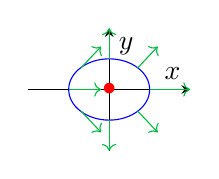
\begin{tikzpicture}
                  \begin{axis}[
                          width=0.3\textwidth,
                          axis lines=middle,
                          no markers,
                          xtick=\empty,
                          ytick=\empty,
                          clip=false,
                          xlabel={$x$},
                          ylabel={$y$},
                          domain=-2:2,
                          ymin=-2, ymax=2,
                          xmin= -2, xmax=2,
                          view = {0}{90}
                      ]
                      \node[red] at (0,0) {$\bullet$};

                      \draw[blue] (0, 0) circle (1);

                      \draw[mygreen, ->] (0:1) -- (0:2);
                      \draw[mygreen, ->] (0.7, 0.7) -- (1.2, 1.4);
                      \draw[mygreen, ->] (90:1) -- (90:2);
                      \draw[mygreen, ->] (-0.7, 0.7) -- (-0.2, 1.4);
                      \draw[mygreen, ->] (-1, 0) -- (-0.2, 0);
                      \draw[mygreen, ->] (-0.7, -0.7) -- (-0.2, -1.4);
                      \draw[mygreen, ->] (0, -1) -- (0, -2);
                      \draw[mygreen, ->] (0.7, -0.7) -- (1.2, -1.4);
                  \end{axis}
              \end{tikzpicture}
          \end{center}

          So $(0, 0)$ has index $0$.

          \color{black}

    \item \quad $\dot{x}=y^3$, \quad $\dot{y}=x$.

          \color{blue}
          \[J(x, y) = \begin{pmatrix}
                  0 & 3y^2 \\
                  1 & 0
              \end{pmatrix} \implies J(0, 0) = \begin{pmatrix}
                  0 & 0 \\
                  1 & 0
              \end{pmatrix} \implies \lambda = 0\]
          \color{black}

          We can graph:
          \begin{center}
              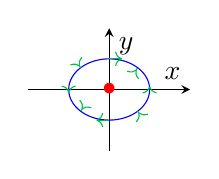
\begin{tikzpicture}
                  \begin{axis}[
                          width=0.3\textwidth,
                          axis lines=middle,
                          no markers,
                          xtick=\empty,
                          ytick=\empty,
                          clip=false,
                          xlabel={$x$},
                          ylabel={$y$},
                          domain=-2:2,
                          ymin=-2, ymax=2,
                          xmin= -2, xmax=2,
                          view = {0}{90}
                      ]
                      \node[red] at (0,0) {$\bullet$};
                      \draw[blue] (0, 0) circle (1);
                      \draw[mygreen, ->, shorten >= 10pt] (1, 0) --  (1, 1); % (0, 1)
                      \draw[mygreen, ->, shorten >= 10pt] (0, 1) --  (1,  1);
                      \draw[mygreen, ->, shorten >= 10pt] (-1, 0) -- (-1, -1);
                      \draw[mygreen, ->, shorten >= 10pt] (0, -1) -- (-1, -1);

                      \draw[mygreen, ->, shorten >= 10pt] (0.7, 0.7) -- (1.05, 1.4);
                      \draw[mygreen, ->, shorten >= 10pt] (-0.7, 0.7) -- (-0.35, 0);
                      \draw[mygreen, ->, shorten >= 10pt] (-0.7, -0.7) -- (-1.05, -1.4);
                      \draw[mygreen, ->, shorten >= 10pt] (0.7, -0.7) -- (0.35, 0);
                  \end{axis}
              \end{tikzpicture}
          \end{center}

          Which has index $-1$.

\end{enumerate}

\pagebreak
%%%%%%%%%%%%%%%%%%%%%%%%%%%%%%%%

\section{Index theory}

We consider $\dot{u}=f(u)$ with $f\in C^1$ and $u\in\R^2$. Suppose that this differential equation has exactly three periodic orbits $\Gamma_1$, $\Gamma_2$, and $\Gamma_3$ that are aligned as indicated below. Assume that all equilibria are hyperbolic (and therefore also isolated). What can you say about their number and their type (attractor, repeller, or saddle) in $\Omega$ and inside $\Gamma_2$ and $\Gamma_3$?

\centerline{\includegraphics[scale=0.8]{Assignment_Figure_5.pdf}}

\color{blue}
By a Theorem from class, every periodic orbit contains at least one equilibrium. Further, the index of a periodic orbit is $1$.

But since $\Gamma_1$ is a simple closed loop, $I(\Gamma_1) = \sum_{i=1}^n I(u_i) = 1$ for each equilibrium $u_i$ in $\Gamma_1$.

In particular, this means that $\Gamma_1$ must contain at least one saddle which is not in $\Gamma_2$ or $\Gamma_3$. Since $\Omega$ can also contain other equilibria, we thus require that $\Omega$ contains one more saddle than attractors/repellers combined.

Meanwhile, $\Gamma_2$ and $\Gamma_3$ can each have:
\begin{itemize}
    \item One attractor or one saddle
    \item $n$ attractors + repellers and $n - 1$ saddles
\end{itemize}
\color{black}

\pagebreak


%%%%%%%%%%%%%%%%%%%%%%%%%%%%%%%%

\section{Trapping regions}

Consider the system
\[
    \dot{x} = a-x+x^2y, \qquad
    \dot{y} = b-x^2y
\]
where $x,y\geq0$ and $a,b>0$.
\begin{enumerate}[(i)]
    \item Find the unique equilibrium of this system.

          \color{blue}
          \[\begin{array}{rl}
                  0 & = a - x + x^2y \\
                  0 & = b - x^2y     \\ \hline
                  0 & = a + b - x
              \end{array}\]

          Hence,
          \[x = a + b \implies y = \frac{b}{x^2} = \frac{b}{(a + b)^2}\]
          so the only equilibrium is $(a+b, b/(a+b)^2)$.
          \color{black}

    \item Determine its stability properties and show that it is not hyperbolic precisely when $(a,b)$ satisfies $b-a=(a+b)^3$.

          \color{blue}
          We have Jacobian
          \[J(x, y) = \begin{pmatrix}
                  -1 + 2xy & x^2  \\
                  -2xy     & -x^2
              \end{pmatrix} \implies J(a + b, \frac{b}{(a + b)^2}) = \begin{pmatrix}
                  -1 + \frac{2b}{a+ b} & (a + b)^2  \\
                  -\frac{2b}{(a + b)}  & -(a + b)^2
              \end{pmatrix}\]

          So,
          \begin{align*}
              \lambda_1 \lambda_2   & = \begin{vmatrix}
                                            -1 + \frac{2b}{a+ b} & (a + b)^2  \\
                                            -\frac{2b}{(a + b)}  & -(a + b)^2 \\
                                        \end{vmatrix} \\
                                    & = (a + b)^2 - 2b(a + b) + 2b(a + b) \\
                                    & = (a + b)^2                         \\
              \lambda_1 + \lambda_2 & = -1 + \frac{2b}{a + b} - (a + b)^2 \\
                                    & = \frac{a - b}{a + b} - (a + b)^2
          \end{align*}

          We have $a, b > 0$ so $\det J > 0$ implies the equilibrium is not a saddle.

          Now, we know the equilibrium is an:
          \begin{itemize}
              \item Attractor if $\frac{b-a}{a + b} > (a + b)^2 $
              \item Repeller if $\frac{b-a}{a + b} < (a + b)^2$
              \item Non-hyperbolic if $\frac{b-a}{a + b} = (a + b)^2$
          \end{itemize}

          Suppose $b - a = (a + b)^3$. Then,
          \begin{align*}
              \frac{b- a}{a + b} - (a + b)^2 & = \frac{1}{a + b}\left(b - a - (a + b)^3\right) \\
                                             & = b - a - (b - a)                               \\
                                             & = 0
          \end{align*}
          which is exactly the condition $\text{tr}\, J = 0$, i.e where the equilibrium is non-hyperbolic.

          \color{black}

    \item Plot the curve determined by $b-a=(a+b)^3$ in the $(a,b)$-plane. \emph{Hint:} Set $v=b-a$ and $u=a+b$, plot the curve in the $(u,v)$-space, and then see what these coordinates and the graph mean in the $(a,b)$-plane.

          \color{blue}
          Let $v = b-a$ and $u = a+b$ so we are interested in the curve $v = u^3$

          \begin{center}
              \color{black}
              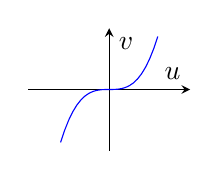
\begin{tikzpicture}
                  \begin{axis}[
                          width=0.3\textwidth,
                          axis lines=middle,
                          no markers,
                          xtick=\empty,
                          ytick=\empty,
                          clip=false,
                          xlabel={$u$},
                          ylabel={$v$},
                          domain=-2:2,
                          ymin=-2, ymax=2,
                          xmin= -2, xmax=2,
                          view = {0}{90}
                      ]
                      \addplot[blue, domain=-1.2:1.2] {x^3};
                  \end{axis}
              \end{tikzpicture}
          \end{center}

          In $(a, b)$-space, this curve corresponds to the line $b - a = (a + b)^3$.

          How do we transform from $(u, v)$ to $(a, b)$? We have $u = a + b$ and $v = b - a$ so
          \[\begin{pmatrix}
                  u \\v
              \end{pmatrix} = \begin{pmatrix}
                  1  & 1 \\
                  -1 & 1
              \end{pmatrix} \begin{pmatrix}
                  a \\b
              \end{pmatrix} \implies \begin{pmatrix}
                  a \\b
              \end{pmatrix} = \frac{1}{2}\begin{pmatrix}
                  1 & -1 \\
                  1 & 1
              \end{pmatrix}\begin{pmatrix}
                  u \\v
              \end{pmatrix}\]
          which happens to be the transformation associated with a rotation by $45^\circ$ and a scaling of $1/\sqrt{2}$.

          \begin{center}
              \color{black}
              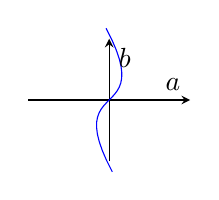
\begin{tikzpicture}
                  \begin{axis}[
                          width=0.3\textwidth,
                          axis lines=middle,
                          no markers,
                          xtick=\empty,
                          ytick=\empty,
                          clip=false,
                          xlabel={$a$},
                          ylabel={$b$},
                          domain=-2:2,
                          ymin=-2, ymax=2,
                          xmin= -2, xmax=2,
                          view = {0}{90}
                      ]

                      \addplot[blue, rotate around={45:(0, 0)}, domain=-1.2:1.2] {x^3};
                  \end{axis}
              \end{tikzpicture}
          \end{center}

          However, we are only interested in the region where $a, b > 0$. What is the b-intercept?
          \[a = 0 \implies b = b^3 \implies b = 1 \; (b > 0)\]

          So we have
          \begin{center}
              \color{black}
              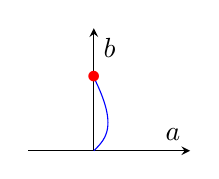
\begin{tikzpicture}
                  \begin{axis}[
                          width=0.3\textwidth,
                          axis lines=middle,
                          no markers,
                          xtick=\empty,
                          ytick=\empty,
                          clip=false,
                          xlabel={$a$},
                          ylabel={$b$},
                          domain=-2:2,
                          ymin=0, ymax=2,
                          xmin=0, xmax=0.5,
                          view = {0}{90},
                          axis equal
                      ]

                      \addplot[blue, rotate around={45:(0, 0)}, domain=0:0.83] {1.4*x^3};
                      \node[red] at (0, 1.2) {$\bullet$};

                  \end{axis}
              \end{tikzpicture}
          \end{center}
          \color{black}

    \item Show that this system has, for appropriate values of $(a,b)$, at least one periodic orbit by constructing a trapping region. This is very similar to (but slightly more involved than) the example we went through in class: be careful and go step-by-step.

          \color{blue}
          We would like for this region (call it $\Omega$) to be a repeller, hence for $(a, b) \in \Omega$, require $\frac{b-a}{a +b } < (a + b)^2$.

          Let's plot nullclines
          \[\begin{cases}
                  \dot x = 0 \implies a - x + x^2y = 0 \implies y = \frac{x - a}{x^2} \\
                  \dot y = 0 \implies b - x^2y = 0 \implies y = \frac{b}{x^2}
              \end{cases}\]

          \begin{center}
              \color{black}
              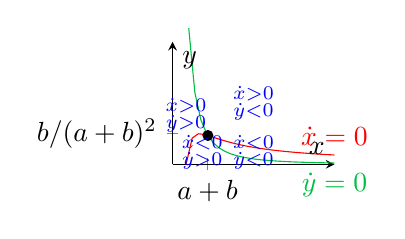
\begin{tikzpicture}
                  \begin{axis}[
                          width=0.3\textwidth,
                          axis lines=middle,
                          no markers,
                          xtick={1.3},
                          ytick={0.5},
                          xticklabels={$a+b$},
                          yticklabels={$b/(a+b)^2$},
                          clip=false,
                          xlabel={$x$},
                          ylabel={$y$},
                          ymin=0, ymax=2,
                          xmin=0, xmax=6,
                          view = {0}{90}
                      ]

                      \addplot[name path=x, domain=0.5:6, red] {(x-0.5)/x^2} node[above] {$\dot x = 0$};
                      \addplot[name path=y, domain=0.6:6, mygreen] {0.8/x^2} node[below] {$\dot y = 0$};

                      \fill [name intersections={of=x and y, by={p}}]
                      (p) circle (2pt);

                      \node[blue] at (3, 1) {$\begin{subarray}{c}
                                  \dot x > 0\\
                                  \dot y < 0
                              \end{subarray}$};

                      \node[blue] at (3, 0.2) {$\begin{subarray}{c}
                                  \dot x < 0\\
                                  \dot y < 0
                              \end{subarray}$};

                      \node[blue] at (1.1, 0.2) {$\begin{subarray}{c}
                                  \dot x < 0\\
                                  \dot y > 0
                              \end{subarray}$};

                      \node[blue] at (0.5, 0.8) {$\begin{subarray}{c}
                                  \dot x > 0\\
                                  \dot y > 0
                              \end{subarray}$};

                  \end{axis}
              \end{tikzpicture}
              \hspace{1cm}
              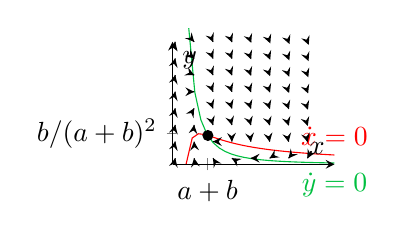
\begin{tikzpicture}
                  \begin{axis}[
                          width=0.3\textwidth,
                          axis lines=middle,
                          no markers,
                          xtick={1.3},
                          ytick={0.5},
                          xticklabels={$a+b$},
                          yticklabels={$b/(a+b)^2$},
                          clip=false,
                          xlabel={$x$},
                          ylabel={$y$},
                          ymin=0, ymax=2,
                          xmin=0, xmax=6,
                          view = {0}{90}
                      ]

                      % a = 0.5, b = 0.8
                      \addplot[name path=x, domain=0.5:6, red] {(x-0.5)/x^2} node[above] {$\dot x = 0$};
                      \addplot[name path=y, domain=0.6:6, mygreen] {0.8/x^2} node[below] {$\dot y = 0$};

                      \fill [name intersections={of=x and y, by={p}}]
                      (p) circle (2pt);

                      \addplot3[samples=8, domain=0.1:5, domain y=0.1:2,
                          quiver={
                                  u={0.5 - x + x^2*y},
                                  v={0.8 - x^2*y},
                                  scale arrows=0.001,
                              }, -stealth] {0};
                  \end{axis}
              \end{tikzpicture}
          \end{center}

          Clearly, the $x$ and $y$ axes will work as two bounds on our trapping region. Now we just need to find lines where the vector field points inwards.

          From part (i), we need $\dot x + \dot y = a  +b - x$. So let's try a slope of $-1$:
          \[\frac{\dot y}{\dot x} < -1 \implies \dot y < -\dot x \implies \frac{b}{x^2} < \frac{x - a}{x^2} \implies b < x - a \implies x >a + b \quad \textcolor{mygreen}{\checkmark}\]

          \begin{center}
              \color{black}

              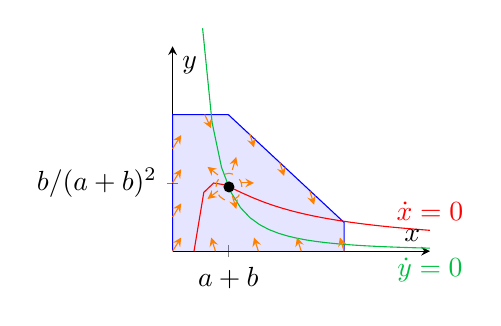
\begin{tikzpicture}
                  \begin{axis}[
                          width=0.4\textwidth,
                          axis lines=middle,
                          no markers,
                          xtick={1.3},
                          ytick={0.5},
                          xticklabels={$a+b$},
                          yticklabels={$b/(a+b)^2$},
                          clip=false,
                          xlabel={$x$},
                          ylabel={$y$},
                          ymin=0, ymax=1.5,
                          xmin=0, xmax=6,
                          view = {0}{90}
                      ]

                      \addplot[fill, fill opacity=0.1, blue] coordinates {
                              (0, 0) (0, 1) (1.3, 1) (4, 0.21) (4, 0)
                          };

                      \addplot[name path=x, domain=0.5:6, red] {(x-0.5)/x^2} node[above] {$\dot x = 0$};
                      \addplot[name path=y, domain=0.7:6, mygreen] {0.8/x^2} node[below] {$\dot y = 0$};

                      \fill [name intersections={of=x and y, by={p}}]
                      (p) circle (2pt);

                      \draw[orange, dashed] (p) ellipse (0.3 and 0.1) ;

                      \pgfplotsinvokeforeach{0, 72, ..., 288}{
                          \draw[orange, -stealth, shift={(1.3,0.5)}] (#1: 0.3 and 0.1) -- (#1: 0.6 and 0.2);
                      }

                      \pgfplotsinvokeforeach{1, ..., 4}{
                          \draw[orange, -stealth] (#1, 0) -- (#1-0.1, 0.1);
                      }

                      \pgfplotsinvokeforeach{0, 0.25, ..., 0.75}{
                          \draw[orange, -stealth] (0, #1) -- (0.2, #1+0.1);
                      }

                      \draw[orange, -stealth] (0.75, 1) -- (0.9, 0.9);

                      \pgfplotsinvokeforeach{1.8, 2.5, ..., 3.8}{
                          \draw[orange, -stealth] (#1, 1.4-0.3*#1) -- (#1+0.1, 1.3-0.3*#1);
                      }


                  \end{axis}
              \end{tikzpicture}
          \end{center}

          By construction, this region is
          \begin{itemize}
              \item Closed and bounded
              \item Does not contain any equilibria
              \item For all $u(0) \in \Omega$, $u(t) \in \Omega$ for all $t \geq 0$
          \end{itemize}

          Hence, by the Poincaré-Bendixson theorem, there must be at least one periodic orbit in $\Omega$.

\end{enumerate}
\pagebreak




\end{document}